\chapter{Implementation}
\label{chap:impl}

\section{System Design}

\subsection{Pull vs. Push Models}

A fundamental architectural decision in distributed orchestration systems concerns the mechanism by which configuration updates and workload instructions are propagated from the control plane to worker nodes. Two predominant paradigms exist: the Push model and the Pull model. These differ not only in data flow direction but also in their underlying philosophy imperative execution versus declarative reconciliation with significant implications for scalability, resilience, and operational complexity.

\begin{figure}[h]
\centering
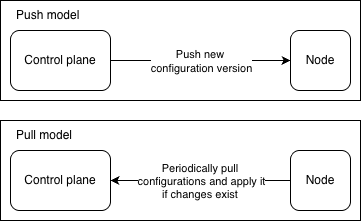
\includegraphics[width=0.8\textwidth]{figs/pull-vs-push.png}

\caption{Comparison of Push and Pull configuration propagation models. In the Push model (top), the control plane initiates outbound connections to apply changes directly to nodes. In the Pull model (bottom), each node periodically polls the control plane or a configuration repository to reconcile its local state with the desired state.}
\label{fig:push-vs-pull}
\end{figure}

The Push model operates imperatively: a central controller initiates synchronous, outbound connections to target nodes to enforce configuration changes immediately upon request. Tools such as Ansible exemplify this approach, often leveraging secure shell (SSH) or Windows Remote Management (WinRM) without requiring persistent agents.

Key advantages include:
\begin{itemize}
\item \textbf{Immediate enforcement}: changes are applied with minimal delay once triggered by an operator.
\item \textbf{Predictable timing}: the operator retains full control over when a change is deployed.
\item \textbf{Simplified auditing}: all modifications originate from a single, identifiable source.
\item \textbf{Reduced node-side footprint}: agentless implementations (e.g., Ansible) avoid long-running processes on worker nodes.
\end{itemize}

However, this model presents notable limitations in large-scale or dynamic environments:
\begin{itemize}
\item \textbf{Scalability bottlenecks}: the central controller becomes a performance bottleneck when managing thousands of nodes concurrently.
\item \textbf{Network constraints}: requires bidirectional connectivity from the controller to every node problematic in environments with firewalls, NAT, or private subnets.
\item \textbf{State drift vulnerability}: nodes that experience local configuration changes or reboots remain out of sync until the next manual or scheduled push.
\item \textbf{Expanded attack surface}: the controller must securely authenticate to all nodes, often necessitating complex credential or key management.
\end{itemize}

In contrast, the Pull model is inherently declarative: each node runs a lightweight agent that periodically (e.g., every 10 seconds) queries a central configuration source such as an API server or Git repository and autonomously reconciles its local state with the declared desired state.

This approach offers several critical benefits aligned with modern reliability engineering principles:
\begin{itemize}
    \item \textbf{Self-healing}: nodes automatically recover from configuration drift or transient failures without external intervention.
    \item \textbf{Horizontal scalability}: load is distributed across nodes; the control plane serves read requests rather than initiating writes.
    \item \textbf{Network resilience}: nodes only require outbound connectivity (e.g., HTTPS to a config server), making the model compatible with restrictive network topologies.
    \item \textbf{Decoupled architecture}: failures in the control plane do not immediately halt node operations; nodes continue functioning with their last known good state.
\end{itemize}

Nonetheless, the Pull model introduces its own trade-offs:
\begin{itemize}
    \item \textbf{Enforcement latency}: configuration changes are applied only at the next polling interval, unless supplemented with event-driven triggers (e.g., webhooks).
    \item \textbf{Agent overhead}: requires a persistent process on each node, increasing resource consumption and attack surface at the edge.
    \item \textbf{Temporal inconsistency}: nodes may operate with slightly divergent configurations until synchronization occurs.
    \item \textbf{Observability complexity}: determining the exact time of state convergence across the fleet requires additional telemetry.
\end{itemize}

Upon thorough analysis, it becomes evident that the requirements established in Section~3.5 particularly the 90-second Recovery Time Objective (RTO), resilience to infrastructure failures, and support for autonomous recovery align closely with the core strengths of the Pull model. The capacity for self-healing, network resilience, and decentralized operation directly addresses the business imperatives of minimizing downtime and reducing manual intervention.

Consequently, the Pull model has been selected as the foundational architectural paradigm for the proposed prototype. Furthermore, the design will incorporate mitigations to address its inherent limitations:

A configurable, short polling interval to bound recovery latency;
Optional event-based push notifications to trigger immediate reconciliation when critical updates occur;
Minimalist agent design to reduce resource footprint;
Centralized telemetry to monitor configuration convergence across the cluster.
This hybrid-aware Pull approach ensures adherence to non-functional requirements while preserving operational simplicity and scalability.

\subsection{Top-Layer Architecture}

Given the explicit non-functional requirements for decentralization, fault tolerance, and automated recovery, the system must be designed from the ground up as a distributed architecture. Modern infrastructure platforms typically decompose into two orthogonal domains: the control plane and the data plane. This separation enables scalability, operational clarity, and independent evolution of concerns.

\begin{figure}[h]
\centering
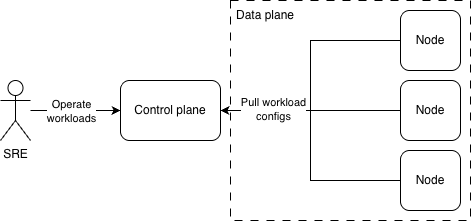
\includegraphics[width=0.8\textwidth]{figs/top-layer-arch.png}
\caption{High-level component diagram of the proposed system. The control plane (central registry) communicates with data-plane nodes via a REST API. Each node runs a local agent that periodically pulls configuration state. An SRE interacts with the control plane to declare desired workload placements.}
\label{fig:component-architecture}
\end{figure}

The control plane serves as the authoritative source of truth for the desired system state. It maintains metadata about workloads (e.g., placement rules, resource constraints, health policies) and exposes interfaces for human (e.g., SRE) and programmatic interaction. Critically, it does not execute user workloads but orchestrates their placement and lifecycle. 

The data plane consists of a fleet of homogeneous infrastructure units - virtual machines, that host and execute actual workloads. These units are treated as cattle, not pets: individually ephemeral and replaceable, but collectively resilient \cite{pets_vs_cattle}.

This clean separation ensures that failures in the data plane do not compromise global coordination, while control-plane resilience mechanisms (discussed below) prevent single points of failure.

\subsection{Control Plane}

The control plane is a mission-critical component: without it, new workloads cannot be scheduled, and failed workloads cannot be rescheduled. To meet the requirement of resilience to control-plane downtime (NFR2), the control plane must be designed as stateless in its compute layer, enabling horizontal scaling and active-active replication across multiple instances.

\subsubsection{Persistent Storage}
A durable, strongly consistent datastore is required to persist the desired state of the system. After evaluation of alternatives (including etcd, Consul, and embedded SQLite), PostgreSQL was selected as the primary storage backend due to the following advantages: open-source and permissively licensed, ensuring cost efficiency and freedom from vendor lock-in; mature, actively maintained, with a large community and enterprise-grade tooling;
ACID-compliant, providing strong consistency guarantees essential for orchestration correctness; widely adopted in production systems, simplifying operational expertise and troubleshooting.

Given the expected workload primarily metadata operations (create, read, update of service definitions) PostgreSQL is more than sufficient in terms of throughput and latency. If scaling limits be approached (e.g., >10k operations/second), the architecture supports migration to PostgreSQL-compatible distributed databases such as YugabyteDB or CockroachDB with minimal application-level changes.

\subsubsection{Application Interface}
To enable communication between the control plane and data-plane agents, a well-defined RESTful API is exposed over HTTPS. While alternatives like gRPC offer superior performance and streaming capabilities, REST was chosen for the following reasons: simplicity of implementation and debugging during the prototype phase; broad tooling support (curl, Postman, standard HTTP clients); sufficient adequacy for the Pull model, where agents perform periodic, low-frequency polling (e.g., every 30 seconds); ease of integration with future API gateway extensions (e.g., authentication, rate limiting).

All techincal API endpoints enforce mutual TLS (mTLS) to ensure confidentiality and authenticity of control-plane communications.

\subsubsection{Ingress}

Since workloads may be scheduled on any node within the data plane, services that require external exposure via HTTP endpoints necessitate a unified ingress point to ensure consistent and discoverable access. To fulfill this requirement, a new dedicated component (henceforth referred to as the Edge) is introduced. The Edge component continuously discovers active workloads that declare HTTP-based network exposure (e.g., via annotations or configuration metadata) and dynamically configures routing rules to proxy incoming requests to the appropriate backend instances over a single, canonical endpoint.

The Edge operates as a lightweight, programmable reverse proxy integrated into the orchestration control plane. While production-grade alternatives such as NGINX or Envoy could serve as drop-in replacements for the Edge component, their adoption would require additional engineering effort to implement real-time synchronization of downstream service endpoints typically achieved through integration with service discovery mechanisms or dynamic configuration APIs (e.g., Envoy’s xDS protocol). For the scope of this prototype, a minimal custom implementation is preferred to maintain architectural simplicity and reduce external dependencies, while retaining the flexibility to migrate to standardized proxy solutions in future iterations.

\subsection{Data Plane}

The data plane comprises the physical or virtual infrastructure units that execute workloads. Consistent with cloud-native principles, these units are homogeneous, ephemeral, and automatically managed  no single node is considered reliable, but the collective ensemble delivers high availability.

\subsubsection{Agent}
Each node in the data plane runs a lightweight agent process, whose responsibilities include:

\begin{itemize}
    \item Periodically polling the control plane’s REST API to retrieve the latest desired configuration
    \item Comparing the desired state with the current local state
    \item Applying necessary changes (e.g., starting/stopping containers, updating network rules)
    \item Reporting node health and workload status back to the control plane
\end{itemize}

The agent embodies the Pull model and enables self-healing: if a node reboots or is replaced, the agent automatically re-synchronizes with the control plane, ensuring eventual consistency.

\subsubsection{Workload Execution}
Workloads are executed in containers to guarantee portability, isolation, and reproducibility across environments. The system uses the Docker Engine as its default container runtime due to its ubiquity, rich ecosystem, and mature tooling. However, the architecture is runtime-agnostic: the agent interfaces with the container runtime via a pluggable abstraction layer (e.g., using the Docker-compatible HTTP API). This design permits future migration to alternative runtimes such as Podman (rootless, daemonless) or CRI-O (Kubernetes-optimized) without modifying core orchestration logic.

Container images are pulled from a secure, authenticated registry, and all runtime configurations (CPU, memory, network) are derived from the declarative specifications stored in the control plane.

This layered, decoupled architecture directly addresses the functional and non-functional requirements:

\begin{itemize}
    \item Fault tolerance via agent-driven self-healing (NFR1)
    \item Control-plane resilience through stateless design and PostgreSQL durability
    \item Scalability via homogeneous data-plane units and REST-based coordination
    \item Security via mTLS and container isolation
\end{itemize}

\subsection{Architecture Finalization}

Having examined each constituent component of the proposed system the control plane, data plane, agent, Edge ingress layer, and their interconnections it is now possible to consolidate these elements into a coherent and implementable architectural blueprint. The resulting design demonstrates strong alignment with both the functional and non-functional requirements established in Section~3.5.

\begin{figure}[h]
\centering
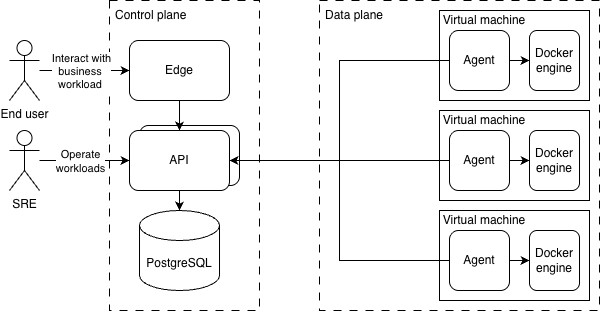
\includegraphics[width=0.8\textwidth]{figs/detailed-arch.png}
\caption{Detailed component diagram of the finalized system architecture, illustrating interactions between the SRE client, control plane (with PostgreSQL backend), data-plane nodes (each running an agent and containerized workloads), and the Edge ingress component.}
\label{fig:final-architecture}
\end{figure}

The design deliberately avoids over-engineering by leveraging lightweight, well-understood technologies (PostgreSQL, REST, Docker) while retaining extensibility for instance, through pluggable runtimes or future integration with mature proxies like Envoy. This balance between simplicity and capability ensures the prototype remains feasible for implementation within the scope of this research, yet representative of real-world operational constraints.

Figure~\ref{fig:final-architecture} presents a comprehensive view of the finalized architecture, capturing data flows, component responsibilities, and communication protocols. This blueprint serves as the definitive reference for the subsequent implementation phase and provides the structural foundation against which the prototype’s correctness and performance will be validated.

\section{Implementation}

\subsection{Technical Scenarios}

